\begin{figure*}[tb]
\centering
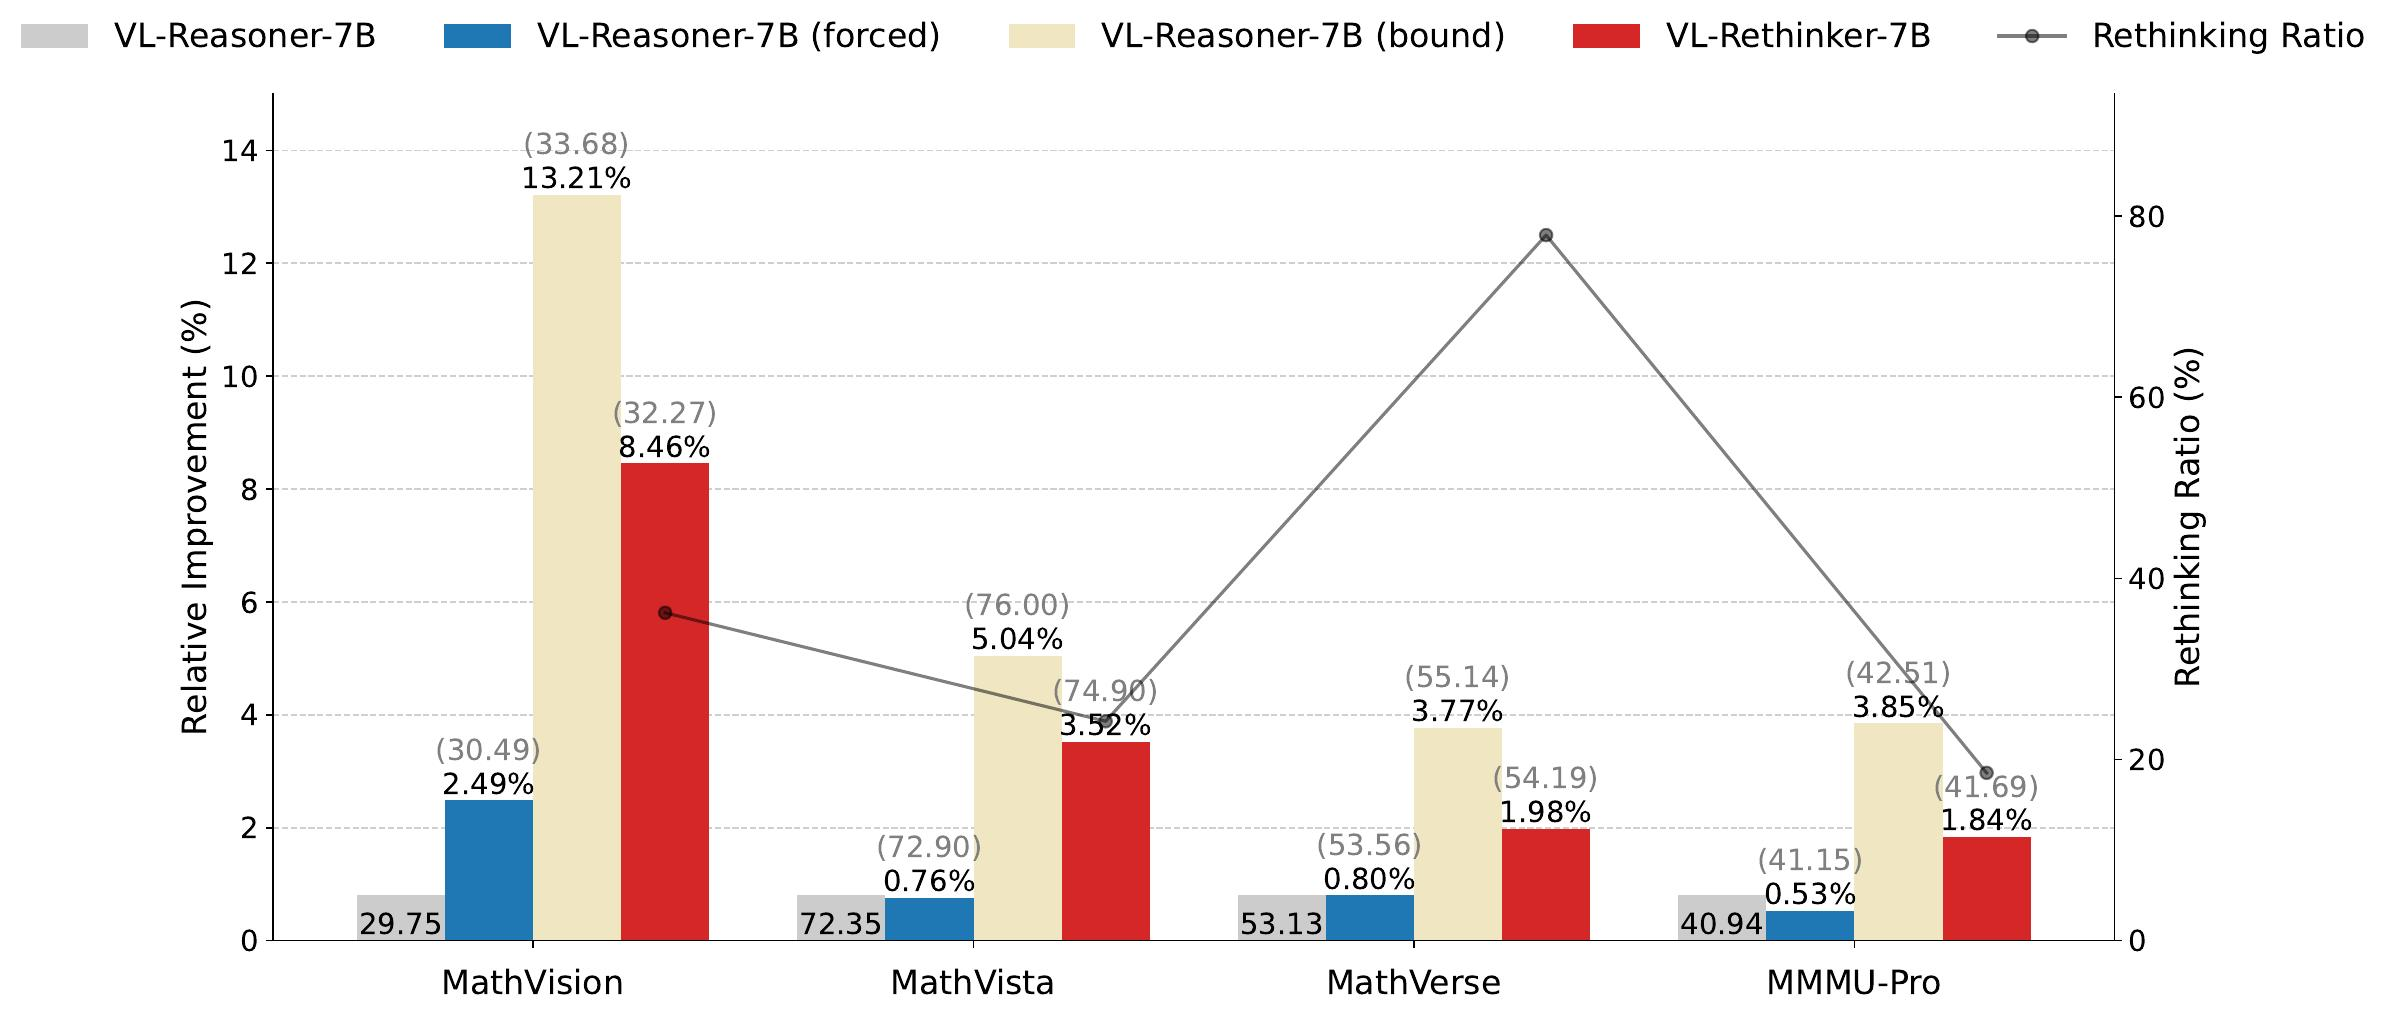
\includegraphics[width=\textwidth]{figures/foret_ablation.jpg}
\caption{\small \textbf{Relative improvement with different rethinking strategies at 7B.} Bars (left axis) give the relative improvement (\%) over VL-Reasoner-7B, the SSR-trained model without Forced Rethinking (gray, its accuracy printed at the bar base). Absolute accuracies are in parentheses. Blue: VL-Reasoner-7B forced to rethink at test time. Beige: an oracle upper bound of test-time rethinking for VL-Reasoner-7B, in which the rethought answer replaces the original only when it is correct. Red: \model-7B, trained with Forced Rethinking. The line (right axis) gives the fraction of \model-7B responses that contain a self-reflection phrase (e.g., ``wait''). Test-time forcing alone gives small gains (0.5--2.5\%), whereas training with Forced Rethinking gives 1.8--8.5\%, with the largest gain on MathVision. \model-7B rethinks selectively rather than uniformly: about 78\% of responses on MathVerse, 36\% on MathVision, and about 24\% and 18\% on MathVista and MMMU-Pro.}
\label{fig:foret_ablation}
\end{figure*}
